

\documentclass[conference]{IEEEtran}

\usepackage[utf8]{inputenc}
\usepackage[pdftex]{graphicx}


\hyphenation{op-tical net-works semi-conduc-tor}


\begin{document}

\title{Técnica de Visualização Computacional Aplicada a Indicadores de Desenvolvimento Humano de Estados e Cidades do Brasil}


% author names and affiliations
% use a multiple column layout for up to three different
% affiliations
\author{\IEEEauthorblockN{Leandro Ungari Cayres}
\IEEEauthorblockA{Faculdade de Ciências e Tecnologia\\
Universidade Estadual Paulista\\
Presidente Prudente, Brasil\\
\textit{leandroungari@gmail.com}}
}



% make the title area
\maketitle

% As a general rule, do not put math, special symbols or citations
% in the abstract
\begin{abstract}
The abstract goes here.
\end{abstract}


\IEEEpeerreviewmaketitle



\section{Introdução}
O conceito de Desenvolvimento Humano objetiva mensurar o avanço de uma população não somente considerando os aspectos de âmbito econômico, mas também características sociais, culturais e políticas que influenciam diretamente na qualidade da vida. A partir desse conceito, o Índice de Desenvolvimento Humano (IDH) foi criado com o intuito de contrapor outro indicador muito utilizado, o Produto Interno Bruto (PIB) per capita~\cite{atlas}.



Mesmo que a utilização do Índice de Desenvolvimento Humano tenha sido realizada em 1990, através de dados demográficos, esse foi recalculado para anos anteriores desde o ano de 1975. Aos poucos, o IDH tornou-se referência e tem sido utilizado pelos governos federal, estaduais e municipais, sob a denominação de Índice de Desenvolvimento Humano Municipal (IDH-M), de forma a apoiar a adoção de políticas públicas e investimentos econômicos para a solução de problemas em contextos sociais específicos.

\section{Fundamentação Teórica}

O IDH é um índice elaborado pela Organização das Nações Unidas usado para medir a qualidade de vida das pessoas em várias regiões do mundo. Nesse indicador, são considerados o PIB per capita (em dólares ajustados ao poder de compra no país), a saúde (medida pela esperança de vida ao nascer) e a educação (considera a taxa de matrícula combinada (peso de $1/3$) com a taxa de alfabetização de pessoas com mais de 15 anos (peso de $2/3$)), todos com pesos idênticos. O resultado é ordenado segundo valores obtidos no cálculo normalizado no domínio entre 0 e 1, sendo a pior e melhor situação de desenvolvimento humano, respectivamente. Segundo o classificador, a região ou país é de alto desenvolvimento quando o IDH é igual ou superior a 0,8; médio, de 0,79 a 0,5, e baixo, de 0,49 ou inferior~\cite{atlas, senak, espn, oxford, araujo}.


\section{Técnica de Visualização}

\begin{figure}[!ht]
\centering
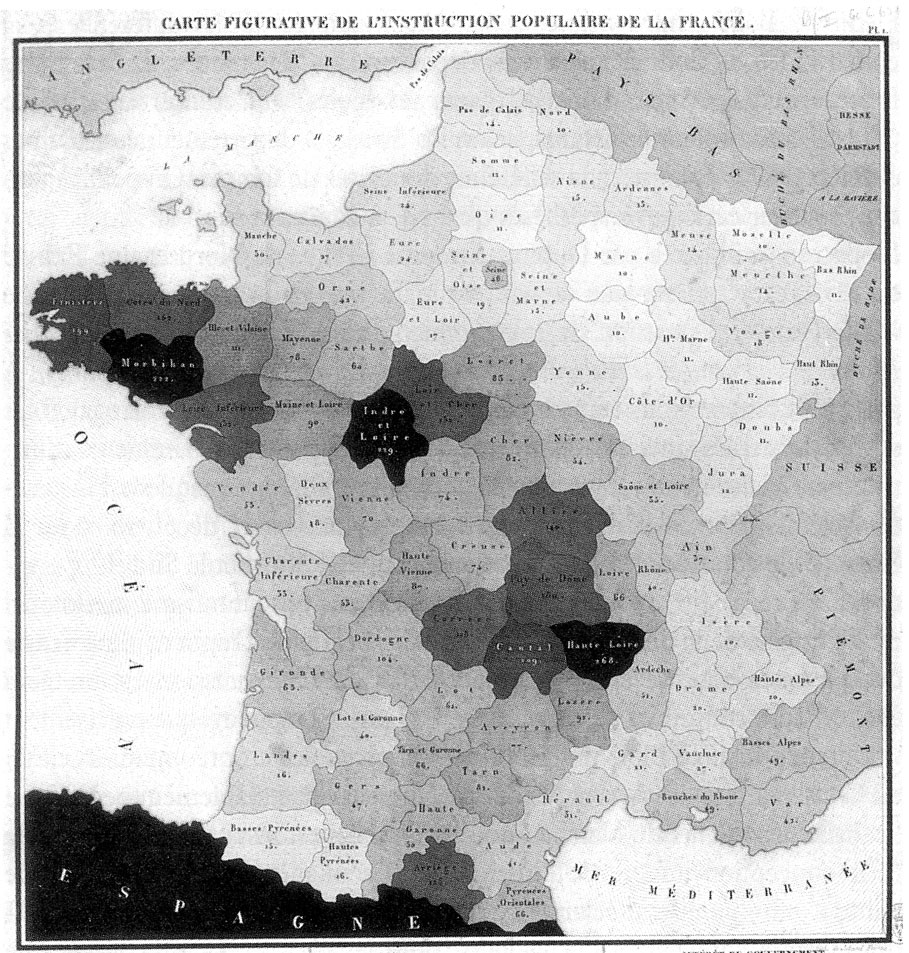
\includegraphics[width=0.4\textwidth]{analfabetismo-franca.jpg}
\caption{Mapa de Analfabetismo na França.}
\label{img:analfabetismo-franca}
\end{figure}


\section{Resultados}

\begin{figure}[!ht]
\centering
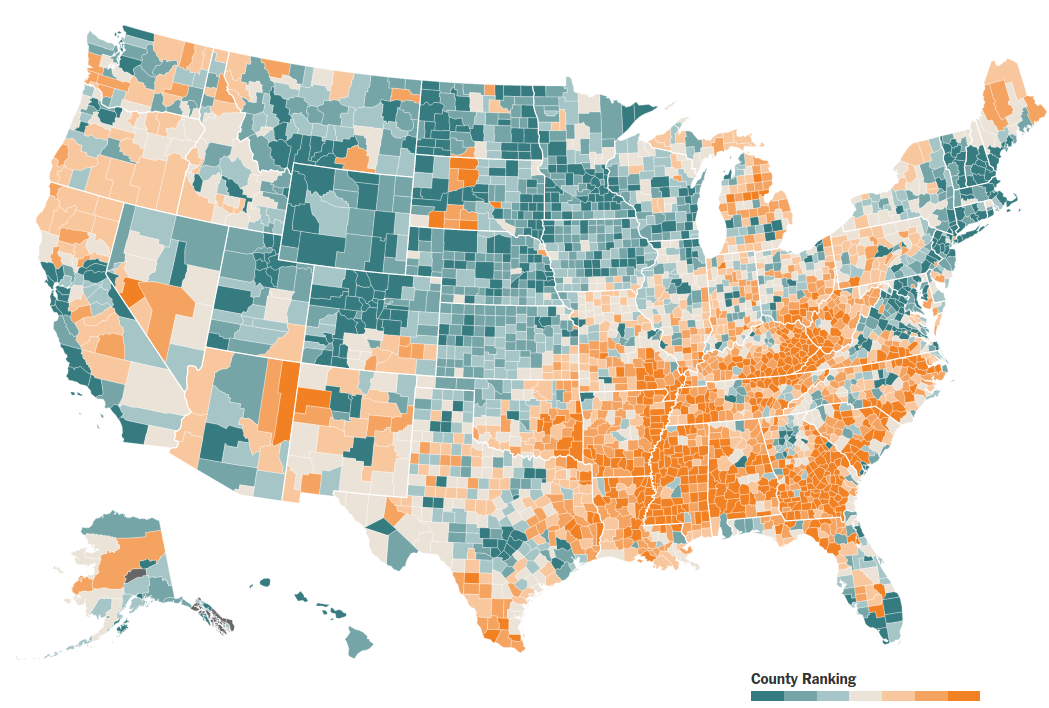
\includegraphics[width=0.40\textwidth]{usa.png}
\caption{Melhores lugares para se viver nos Estados Unidos.}
\label{img:lugares-viver-usa}
\end{figure}



\section{Conclusion}
The conclusion goes here.




% conference papers do not normally have an appendix


% use section* for acknowledgment
\section*{Acknowledgment}


The authors would like to thank...




\begin{thebibliography}{1}


\bibitem{atlas}
Programa das Nações Unidas para o Desenvolvimento (PNUD). \emph{Atlas do desenvolvimento humano do Brasil}. PNUD; 2003. Disponível em: http://www.pnud.org.br/atlas/

\bibitem{senak}
Sen AK. \emph{Desenvolvimento como liberdade}. São Paulo: Companhia das Letras; 2000.

\bibitem{espn}
Programa das Nações Unidas para o Desenvolvimento (PNUD). \emph{Informe sobre desarrollo humano: profundizar la democracia en un mundo fragmentado}. Espanha: Ediciones MundiPrensa; 2002.

\bibitem{oxford}
Programa das Nações Unidas para o Desenvolvimento (PNUD). \emph{Human development report: Millennium Development Goals: A compact among nations to end human poverty}. New York: Oxford University Press; 2003.

\bibitem{araujo}
Araujo PRM. \emph{Charles Taylor: para uma ética do reconhecimento}. São Paulo: Loyola; 2004


\end{thebibliography}




% that's all folks
\end{document}


